\documentclass[crop,tikz]{standalone}

\usepackage[utf8]{inputenc}

% 'crop' is the default for v1.0, before it was 'preview'
%\usetikzlibrary{...}% tikz package already loaded by 'tikz' option

\begin{document}

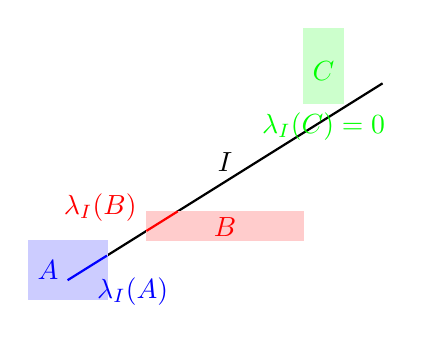
\begin{tikzpicture}

	%the actual segment
	\draw[thick] (0,0) -- (4,2.5);
	\node[anchor=south] at (2,1.25) {$I$};
	
	%area of some set A (blue)
	\filldraw[blue!20!white] (-0.5,-0.25) rectangle (0.5,0.5);
	\node[color=blue, align=center] at (-0.25,0.125) {$A$};
	\draw[thick, color=blue] (0,0) -- (0.5,2.5/8);
	\node[color=blue, anchor=north west] at (0.25,1.25/8) {$\lambda_I(A)$};
	
	%area of some set B (red)
	\filldraw[red!20!white] (1,0.5) rectangle (3,0.875);
	\node[color=red, align=center] at (2,0.675) {$B$};
	\draw[thick, color=red] (1,2.5/4) -- (4*0.875/2.5,0.875);
	\node[color=red, anchor=south east] at (1,2.5/4) {$\lambda_I(B)$};
	
	%area of some set C (green) with zero measure
	\filldraw[green!20!white] (3,2.25) rectangle (3.5,3.2);
	\node[color=green, align=center] at (3.25,2.65) {$C$};
	\node[color=green, anchor=north] at (3.25,2.25) {$\lambda_I(C)=0$};
\end{tikzpicture}

\end{document}